\documentclass[a4paper,twocolumn]{article}
%\documentclass[a4paper]{article}
\usepackage{graphicx}
\usepackage{caption}
\usepackage{subcaption}
\usepackage{dblfloatfix}
\usepackage{fixltx2e}
\usepackage{url}
\usepackage{amssymb}
%\usepackage{natbib}

%\addbibresource[<options for bib resources>]{<mybibfile>.bib}


%Set up title
\author{Idris Miles\\
Bournemouth University SDAGE level I}
\title{Local Avoidance Techniques for Real-Time Crowd Simulation}
\date{\today}

%begin the document
\begin{document}

\maketitle

\section*{Abstract}
In this paper I demonstrate the use of Reciprocal Velocity Obstacle, RVO, as a viable local avoidance model for real time agent based crowd simulation. \\

\section{Introduction}
Crowd simulation is a growing niche for films in the animation and VFX world, where complete CG worlds are brought to life with their own CG inhabitants. Of course it would be too much to ask animators to animate the 300 pedestrians in the background, or the thousands of fans in a sports arena. So the use of crowd simulation tools were bought to life. There are many different aspects involved in crowd simulation: behaviour of the characters, also known as agents, global navigation of the agents, local obstacle avoidance, the animation system, so the characters don't glide around, physics if you want characters to react appropriately to various effects, the list goes on.

\section{Local Avoidance in Crowd Simulation}
Local avoidance is the avoidance of agents within a close proximity of each other, it is useful when there are multiple moving objects in the world that the global navigation system may ignore, due to the fact their position is constantly changing. Global navigation differs from local avoidance because it looks at finding a route from one location to another, while local avoidance just considers its surroundings and desired direction and aims to avoid collisions while staying on track to its goal. Artificial Intelligence also differs from local avoidance although the two can be linked together, AI focuses on creating behaviours of the agents such as forming groups or separating from other types of agent/objects in the virtual world. AI can indirectly incorporate local avoidance due to the behaviours it may create but often this isn't enough to satisfy a collision free system, hence local avoidance can be 'layered' on top. Boids flocking and social forces are examples of behaviour that can result in indirect local avoidance however they are not enough on their own to guarantee it. Reciprocal Velocity Obstacle, RVO, is not a behaviour but is purely a form of local avoidance. It is the RVO technique that is the main focus of my project.\\

\section{Initial Research}
\begin{figure}
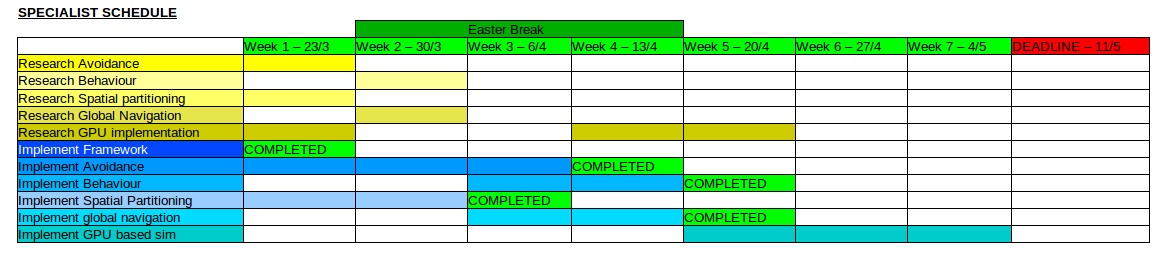
\includegraphics[scale=0.2]{../schedule/specialistSchedule.png}
\caption{Project Schedule}
\label{fig:schedule}
\end{figure}

\begin{figure}
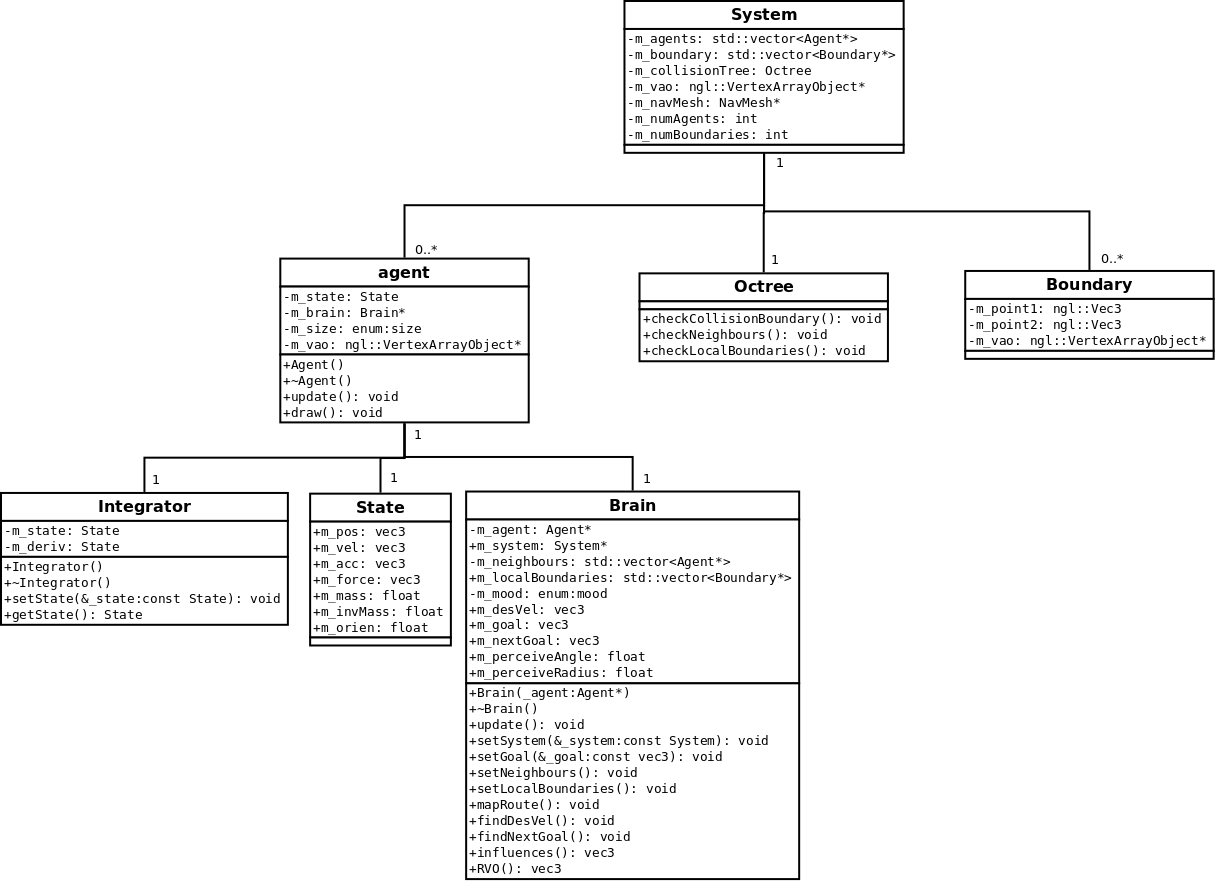
\includegraphics[scale=0.13]{../umlDiagram/Agent_UML_diagram.png} 
\caption{UML class diagram}
\label{fig:umldiagram}
\end{figure}
The first call of action was to make a time schedule that I would follow in order to keep on track, as time management would be crucial in this project. Figure \ref{fig:schedule} shows this in the form of a gant graph.
For my initial research I looked into the various methods used for local avoidance and what techniques current systems used. The main methods I came across were Boids Flocking System\cite{CRBF}, Social Forces and Reciprocal Velocity Obstacle. I felt flocking was not suitable as it was better for replicating animal behaviour such as birds rather than humans. Social forces is an interesting technique that is better for producing human behaviours but not necessarily guaranteed object avoidance. Reciprocal Velocity Obstacle, RVO, is a method not so focused on the behaviour of the agent but rather aims to choose an appropriate velocity that will not result in a collision. RVO is a technique used in various systems including Goalem crowd plugin for Maya and Unreal Engine 4. I decided to focus on the use of RVO as it seemed the most suitable for my project.\\
Figure \ref{fig:umldiagram} shows my initial UML diagram of how I felt my code would be structured, to do this I looked into design patterns \cite{OODPWS}\cite{GPDSWS}.\\


\section{RVO}
RVO  is an agent based method for collision avoidance and was developed by Jur Van Den Burg et all \cite{JBerg2008RVO}. It is based upon a similar technique known as Velocity Obstacle (VO), and uses much of the same principle but with some critical tweaks, which was initially designed for motion planning of autonomous robots. However these techniques have been extended for use in crowd  simulation.\\


\subsection{How RVO Works}
\begin{figure}[b]
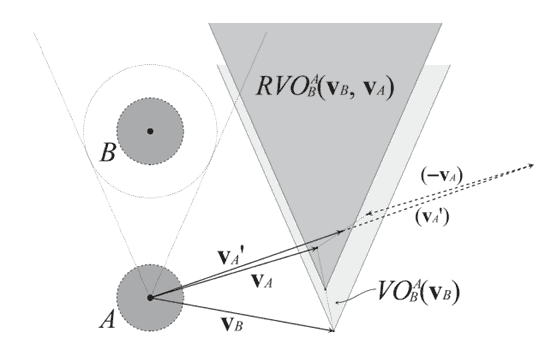
\includegraphics[scale=0.4]{images/rvoDiagram.png}
\caption{Velocity Obstacle cone generated during RVO}
\label{fig:rvoCone}
\end{figure}

\begin{center}
\begin{figure*}[t]
\centering
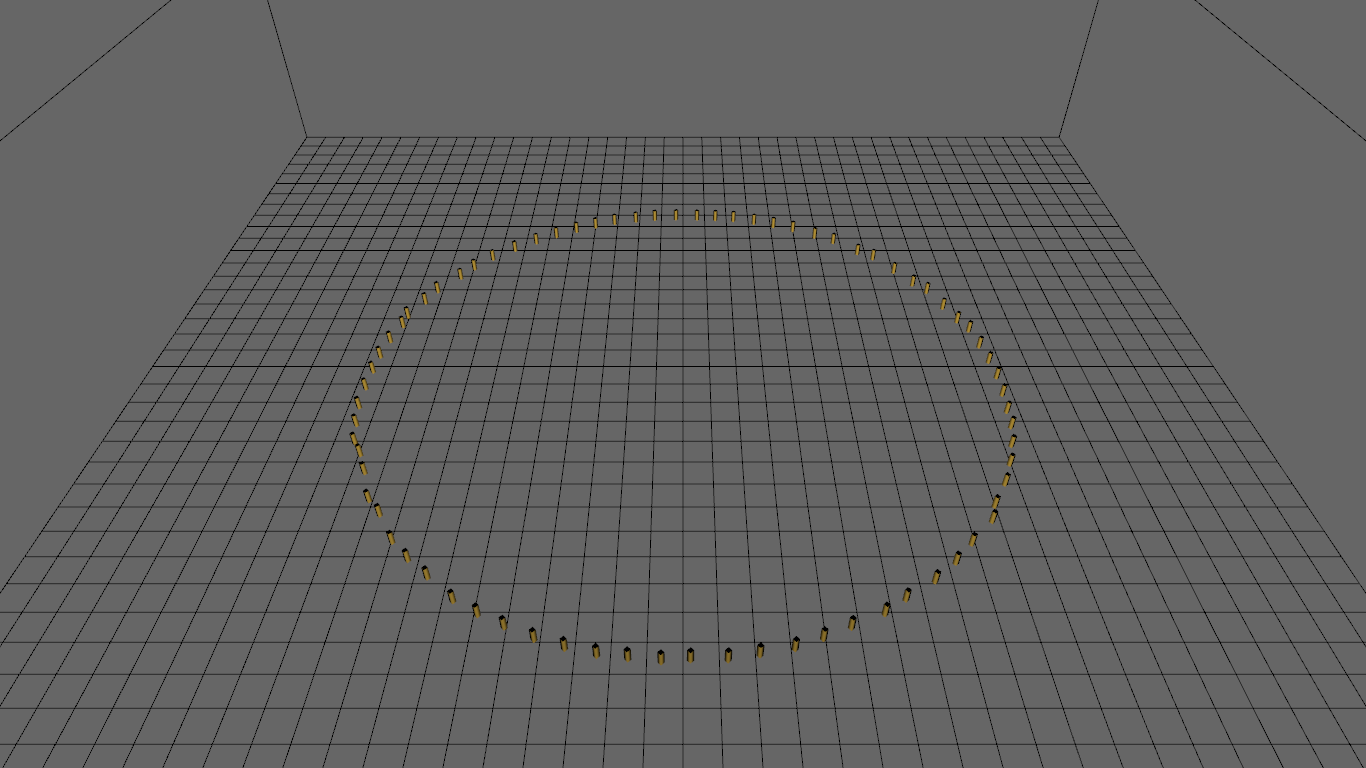
\includegraphics[scale=0.08]{images/RVO_circle.png}
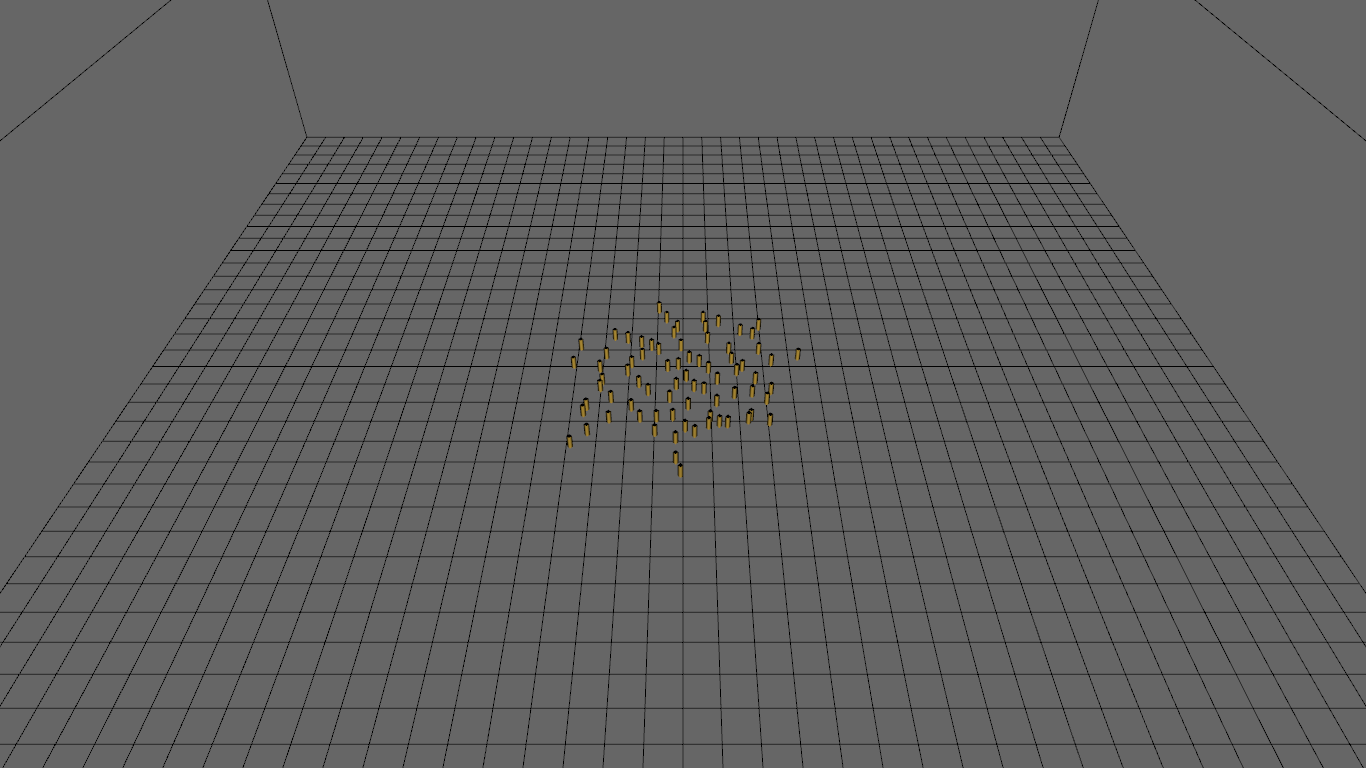
\includegraphics[scale=0.08]{images/RVO_circle2.png}
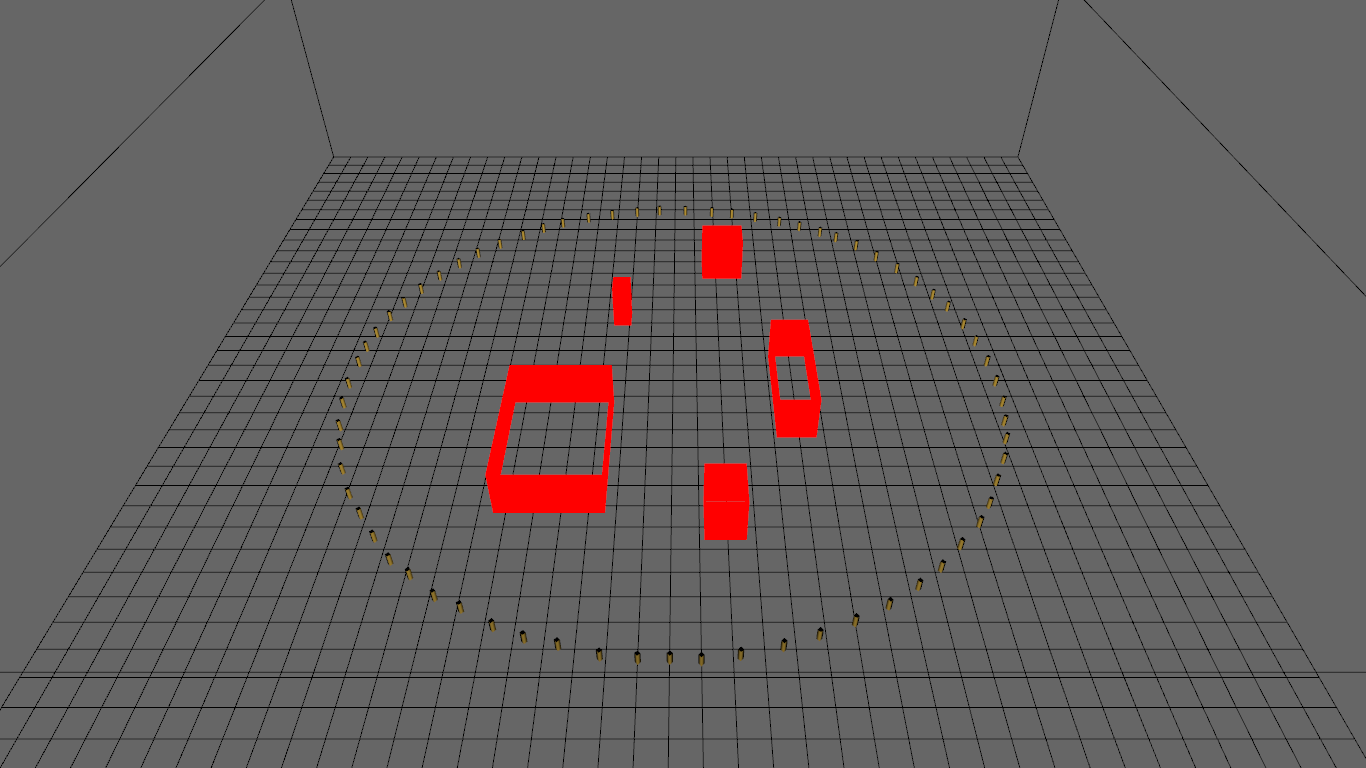
\includegraphics[scale=0.08]{images/RVO_bounds_circ.png}
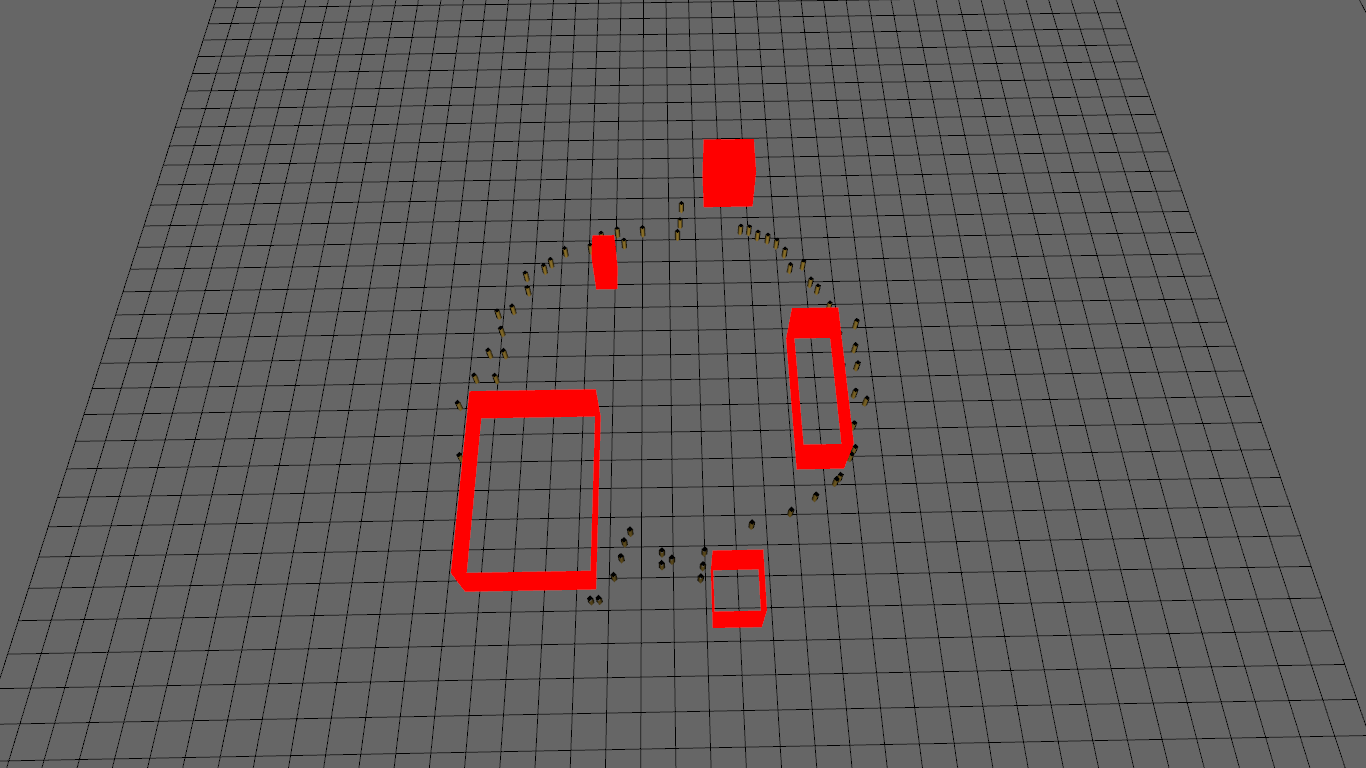
\includegraphics[scale=0.08]{images/RVO_bound_circ2.png}
\caption{RVO avoidance with 100 agents in a circle}
\label{fig:RVOcircle}
\end{figure*}
\end{center}


VO, which RVO is based from, works by the following:\\
\begin{center}
$VO^{A}_{B} (v_{B} ) = \{v_{A} | λ(p_{A} , v_{A} − v_{B} ) \cap B \oplus − A = \varnothing \}$
\end{center}

This translates to, the velocity obstacle $VO^{A}_{B} (v B )$ of agent \emph{B} to \emph{A} is the set of velocities $V_{A}$ for \emph{A} that will result in a collision with \emph{B} moving at velocity $V_{B}$. The idea is to find a new velocity for the agent \emph{A} that is outside the VO of \emph{B}. The difference with RVO and VO is instead of finding a velocity outside the VO of \emph{B} we find the average between the velocity outside and the current velocity \cite{JBerg2008RVO}\cite{AGuy2009CP}, this can be seen in figure \ref{fig:rvoCone}. This produces smoother movement of the agent and guarantees oscillation free movement which can be a common problem for local avoidance.\\

\subsection{RVO Implementation}
My implementation works by first creating the sample velocities according to the desired velocity. Then iterate through each velocity, within each iteration we also loop through all the neighbours. Inside this second loop we perform RVO. First we create the VO cone, then we check the current test velocity and if it intersects with the VO we find the time to collision, \emph{t}, and store it in an array for analysis later, however if the velocity does not collide we return a \emph{true} value that is stored in another array. If for all agents tested against the current test velocities return \emph{true} we can exit all loops and accept the test velocity, however if this is not the case we move onto the next velocity and repeat. In the case of no velocity being directly acceptable we work out each of the penalty values to determine the best velocity\cite{DCherry2013RVO}\cite{JBerg2008CS}.\\


\section{Optimizations}
Using hash table and Moving heavy computation to a compute shader. \cite{NOthman2013SP}
The first optimization I implemented was incorporating a hash table. The hash table speeds up the neighbour search considerably, rather than being of $O(n^{2})$ time complexity it becomes $O(n)$. A further optimization is to have the agent only search half the necessary neighbouring hash table cells, when it finds a neighbour each agent adds each other to their neighbour list. This means that half the number of neighbour queries have to be completed.\\
The next optimization was not for speed increase but rather refining RVO. During times when the crowd became dense the agents could become very conservative with their movement, this is due to the shape of the VO cone. The tip of the cone can be cut so that we have 3 edges to check against rather than 2\cite{AGuy2009CP}, although increasing the number of calculations it also increases the available velocities for the agent. In the case of a velocity being selected due to having the smallest penalty value, it is multiplied by \emph{t}, the time to collision, this means we can slow down the agent. This is not perfect as it means some optimal velocities may be overshadowed however it is a quick method which is necessary for real-time applications.\\

\section{Conclusion and Future Work}
I am pleased with the outcome of the project as I feel I was successful in investigating local avoidance techniques focusing on real-time requirements. My implementation is proof off the success of my research as my simulation works. Future work will entail adding global navigation through the use of A* path finding as well as incorporating more complex behaviour such as a refined social forces model. I would also like to further optimize my simulation through GPGPU, certain parts of the program such as the nearest neighbour search on the hash table can be accomplished in parallel\cite{GGHT}.\\


%\bibliographystyle{plainnat}
\bibliographystyle{plain_annote}
\bibliography{references}

% this is because each agent is put into a "bucket" that is associated with its position, the hash table consists of an array of these "buckets", and to find the agents neighbours you simply have to query the "bucket" the agent belongs to and the neighbouring "buckets". 


Report word count: \emph{x}\\
Annotated bibliography word count: \emph{x}

\end{document}
